\section{Metodologia}

\subsection{Introdução a Linguagem de Programação Matemática}

\subsection{Hipóteses e definições da formulação do problema}

\begin{figure}[H]
    \centering
    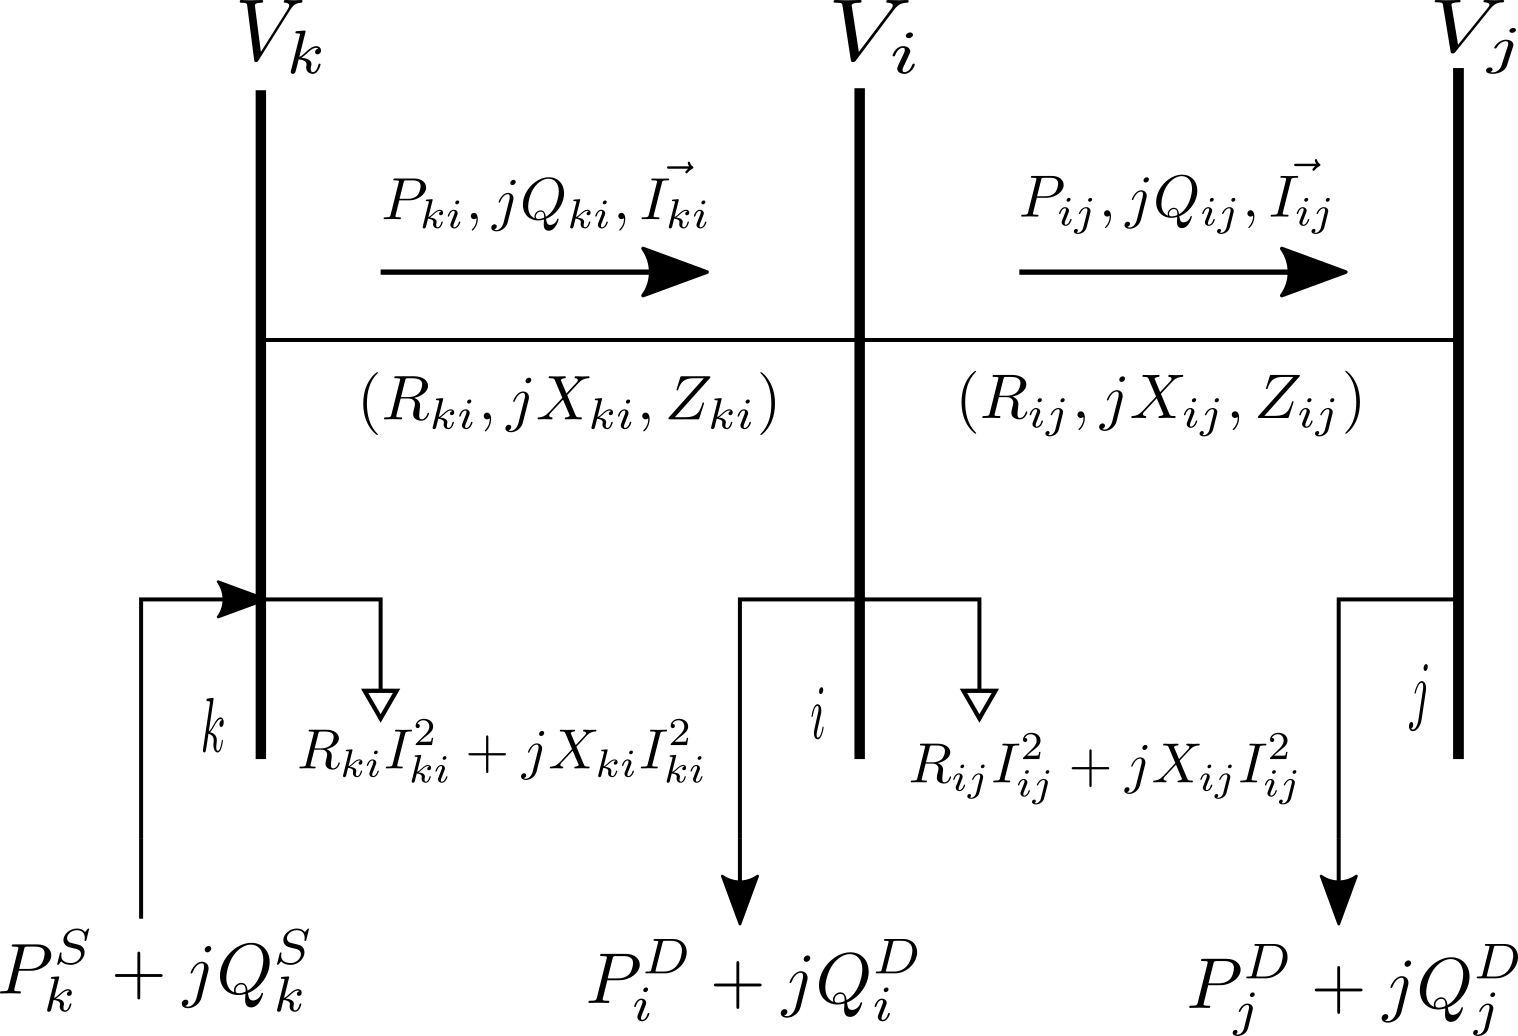
\includegraphics[scale = 1.2]{01_img/diagrama_nos.png}
    \caption{Sistema de distribuição radial}
    \label{fig:SDR}

\end{figure}

Hipóteses adotadas:
Visando representar o funcionamento em regime permanente de um sistema de distribuição de energia, são feitas as seguintes hipóteses (comumente usadas nas formulações de varredura de fluxo de carga \cite{ShirmohammadiANetworks} e mostradas na figura \ref{fig:SDR}.

\begin{itemize}
    \item As demandas nas cargas na rede de distribuição são representadas como potência ativa e reativas contantes;
    
    \item O sistema é balanceado e representado pelo seu equivalente monofásico;
    
    \item As perdas de potência ativa e reativa no circuito \textit{ij} estão concentradas no nó \textit{i}.
    
    \item As chaves são representadas como circuito curtos de impedância nula.
\end{itemize}